\chapter{Threat Model}

Security as part of a software project is nowadays an element that should no longer be neglected. When security is considered from the beginning of a project, it is much easier to keep pace of the evolving threat landscape, quickly derive implications in case of an emerging vulnerability and adapt the project where necessary. Another benefit is the significantly shorter time to react as identifying the project's exposure is faster and easier with a constantly kept up-to-date threat model.

Writing secure software starts with the awareness of the various threats a project might exposed to. This includes applications, interfaces, hardware and users, where potential vulnerabilities can impact the reliability and integrity of a system. If the developer team sticks to the practice of continually updating the threat model and implementing security features as part of each deployment, security can actually become a fun topic and an important feature of the project.

\section{Track Thread Review}
The table \ref{tab:threat-review} lists all risk reviews.

\begin{table}[h!]
  \centering
  \caption{\label{tab:threat-review}Threat Reviews and Changelog}
  \begin{tabular}{ | l | l | }
    \hline
    \textbf{Date} & \textbf{Changes} \\
    \hline
    03.03.22 & Created initial analysis. \\
    \hline
    14.03.22 & Threats reviewed. Nothing changed. \\
    \hline
    31.03.22 & Threat reviewed. More detailed analysis. \\
    \hline
    02.04.22 & Threats reviewed. Adapted architecture.\\
    \hline
  \end{tabular}
\end{table}

\section{STRIDE}

For KubeWatch we define our threat model based on the STRIDE model.
\begin{itemize}
    \item [{\bfseries S}]poofing (Authenticity)
    \item [{\bfseries T}]ampering (Integrity)
    \item [{\bfseries R}]epudiation (Non-Repudiation)
    \item [{\bfseries I}]nformation disclosure (Confidentiality)
    \item [{\bfseries D}]enial of Service ( Availability)
    \item [{\bfseries E}]levation of privilege (Authorisation)
\end{itemize}


\section{Architecture and Trusted Boundaries}

\begin{figure}[h]
    \centering
    \caption{\label{fig:threat-model-architecture}Threat Model Architecture}
    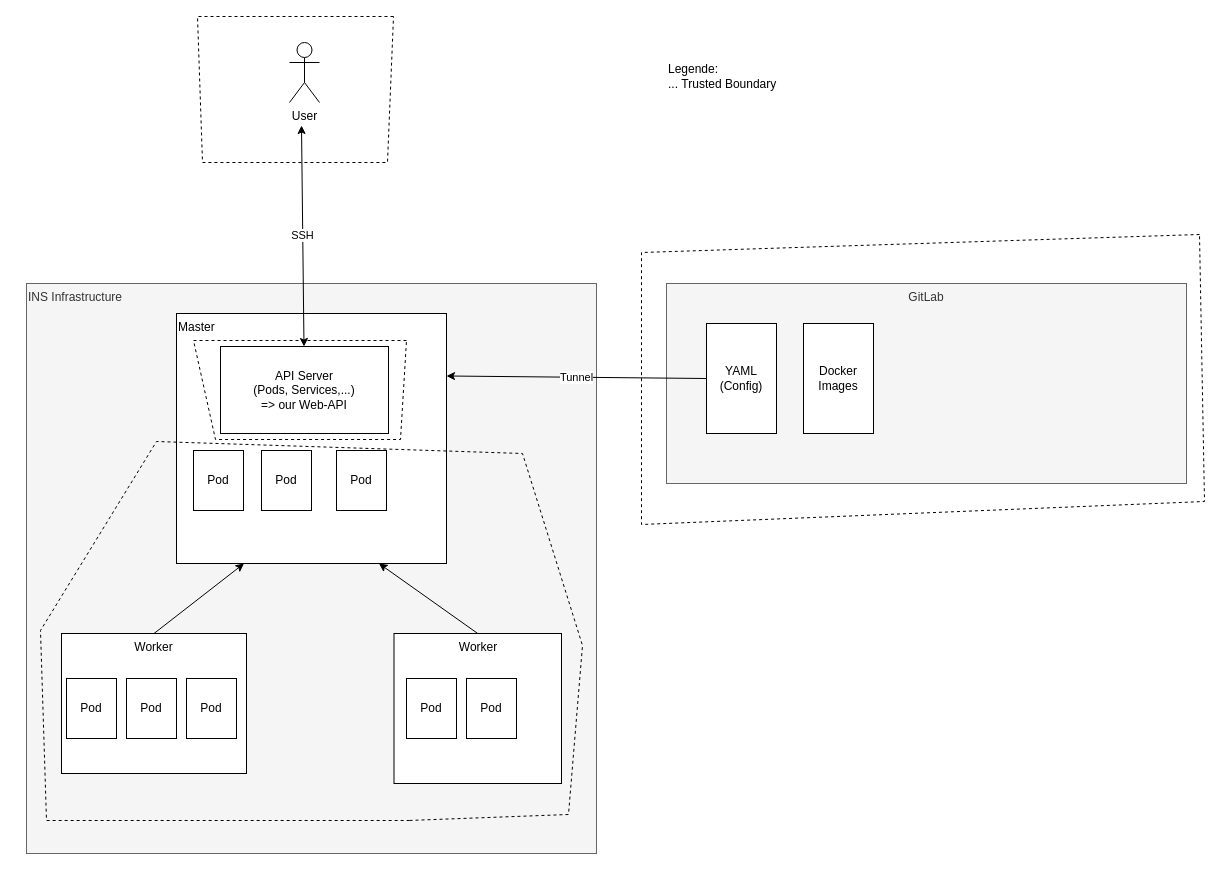
\includegraphics[height=12cm]{resources/architecture_threat_model.png}
\end{figure}
Legend: \newline
- - - Trusted Boundaries


\newpage
\section{Threat Identification}
The following table includes all threats that we found in our architecture and are categorized in the STRIDE model categories.
\begin{longtable}[h!]{p{2.1cm} p{1.8cm} p{3cm} p{2cm} p{3.5cm}}
    \textbf{Component} & \textbf{Category} & \textbf{Threats} & \textbf{Risk} & \textbf{Mitigation} \\ \hline
    \endhead
    \caption{\label{tab:threats-classification}Classification of identified threats}
    \endlastfoot
    User                & D, E & Worm & Low & Anti-virus / Anti-malware\\
                        & & Residual risk & Low & \\
    \hline
    User \(\leftrightarrow\) Frontend   
                        & T & Redirects Data Flow & Low & Use certificate on web server \\ 
                        & I & Eavesdropping & Medium & Data Encryption \\
                        & I & NoSQL Injection & High & Input validation \\
                        & D & Website Defacement & Low & ACL and Filtering \\
                        & D & Botnet Attack & High & CDN and redundant system \\
                        & & & & Patch Services \\
    \hline
    Frontend            & S & Session Hijacking & Medium & Install SSL certificate \\
                        & T & XSS & Medium & Input validation, alert system, santisation \\
                        & R & Audit Log Deletion & Low & Backup audit log \\
                        & R & Insecure Backup & Low & Implement digital signature and encryption \\
                        & I & NoSQL Injection & High & Input validation \\
                        & I & Verbose Exception & Medium & Correct exception handling, no critical information disclosure \\
                        & D & Website Defacement & Low & ACL and Filtering \\
                        & D & Botnet Attack & High & CPU limitation, CDN and redundant system \\
    \hline
    Frontend  \(\leftrightarrow\) KubeWatch Backend API
                        & T & Redirects Data Flow & Low & Use certificate on web server \\
                        & I & NoSQL Injection & High & Input validation \\
                        & D & Botnet Attack & High & CDN and redundant system \\
    \hline
    KubeWatch Backend API
                        & S & Session Hijacking & Medium & Install SSL certificate \\
                        & T & XSS & Medium & Input validation, alert system, sanitisation \\
                        & R & Audit Log Deletion & Low & Backup audit log \\
                        & R & Insecure Backup & Low & Implement digital signature and encryption \\
                        & I & NoSQL Injection & High & Input validation \\
                        & I & Verbose Exception & Medium & Correct exception handling, no critical information disclosure \\
                        & D & Server Defacement & Low & ACL and Filtering \\
                        & D & Botnet Attack & High & CPU limitation, CDN and redundant system \\
    \hline
    KubeWatch Backend API \(\leftrightarrow\) Database
                        & T & XSS & Medium & Input validation, alert system, sanitisation \\
                        & I & NoSQL Injection & High & Input validation \\
                        & I & Verbose Exception & Medium & Correct exception handling, no critical information disclosure \\
    \hline
    Database            & T & XSS & Medium & Input validation, alert system, sanitisation \\
                        & R & Audit Log Deletion & Low & Backup audit log \\
                        & R & Insecure Backup & Low & Implement digital signature and encryption \\
                        & I & NoSQL Injection & High & Input validation \\
                        & I & Verbose Exception & Medium & Correct exception handling, no critical information disclosure \\
                        & D & Botnet Attack & High & CPU limitation, CDN and redundant system \\
    \hline
    KubeWatch Backend API \(\leftrightarrow\) Prometheus
                        & T & XSS & Medium & Input validation, alert system, sanitisation \\
                        & I & NoSQL Injection & High & Input validation \\
                        & I & Verbose Exception & Medium & Correct exception handling, no critical information disclosure \\
    \hline
    Prometheus          & S & Session Hijacking & Medium & Install SSL certificate \\
                        & R & Audit Log Deletion & Low & Backup audit log \\
                        & R & Insecure Backup & Low & Implement digital signature and encryption \\
                        & T & Metrics manipulation & Low & Use secure channel / tunnel \\
    \hline
\end{longtable}


\section{Model Assumptions and Explanations}

\subsection{User}
\begin{itemize}
    \item Assumption: The user has read-only access to the web application because he just needs to look at the cluster metrics.
    \item In the next step when the user needs to change some data the login will be required and then the threat model needs to be updated to the authentication.
\end{itemize}


\subsection{Interface: User \(\leftrightarrow\) Kubernetes Master}
\begin{itemize}
    \item Assumption: the web app is only accessible from within INS.
    \item SQL Injection between Web App and database: mainly information disclosure, potentially Tampering to misrepresent the state of the nodes which are under a denial of service attack. This could pretend that the nodes are up and healthy, while the cluster is actually going down. However, the likelihood of this type of attack is rather low as it is questionable what the benefits are for an attacker. Unless there is a critical application running that may be the target.
    \item SSH connection between a user and K8s cluster: keep ssh service up to date, especially any TLS implementations to ensure authenticity and integrity.
    \item Potential extension: external web app / domain reqired \(\rightarrow\) requires user authentication \(\rightarrow\) update Threat model.
\end{itemize}

\subsection{API Server on Master}
\begin{itemize}
    \item A Master under DoS attack would prevent the API and the Server from running
        \begin{itemize}
            \item This is a dependency on the Master
            \item Mitigation: CPU limitation and alert to users
        \end{itemize}
    \item Potential extension of the threat model: if Web App is externally accessible user authentication is required to ensure only authorised users can access the monitoring and potentially the cluster data
\end{itemize}

\subsection{Cluster}
\begin{itemize}
    \item In-Cluster communication: how does the Master communicate with the Workers and the various Nodes?
    \item Potential extension of the threat model: depending on the protocol used the model has to take threats targeting this communication into account
\end{itemize}

\subsection{Interface Master \(\leftrightarrow\) GitLab}
\begin{itemize}
    \item Tunnel between the Master / Cluster and the GitLab pipeline is assumed to be low risk due to the default secure implementation nature of a tunnel. Of course, the same security issues for any component using TLS apply here as well.
\end{itemize}

